\chapter{微分流形}

微分流形是微分几何的核心对象, 也是我们在本章中要重点讨论的对象.
我们了解了拓扑流形, 接下来我们要在拓扑流形的基础上, 加入一些微分结构, 从而得到微分流形.

如果你熟悉{\bf 层论} (sheaf theory) 的话, 微分流形无非是一种赋环空间
$(M,\mathcal O_M)$, 其中 $M$ 是一个拓扑流形, $\mathcal O_M$ 则是由 $C^\infty$ 函数构成的层.
我们会在de Rham上同调的讨论中回到并更进一步讨论这个定义的优势.

但我们在本章中并不打算使用层论的语言, 因此我们将从一个更为直观的角度来定义微分流形.

\section{基本概念}

\subsection{定义微分流形}

我们现在手上有拓扑流形这个工具, 他满足每个点都存在邻域和 $\R^n$ 同胚, 
但这样定义的拓扑流形很可能是粗糙不堪的, 这并不符合我们的美学, 
我们的想法是在上面附加一种能够描述光滑结构的东西, 从而得到微分流形.

在欧氏空间中, 我们知道如何定义光滑函数[\ref{def:smooth_function}], 
以及光滑函数的微分, 以及微分的链式法则等. 仿照我们定义拓扑流形的哲学,
我们可以在每个点的邻域上定义一个光滑结构, 也就是说, 在每个点的邻域上定义一个同胚到 $\R^n$ 的图册.

我们想更进一步讨论流形的坐标卡, 我们知道坐标卡本质是一个邻域 $U$ 和同胚映射 $\phi$ 的二元组.
其中
\[\phi:U\to\phi(U)\hto\R^n\]
是同胚, 此时对于点 $p\in U$, 我们称
\[\Big(\,\pi_1(\phi(p)),\ldots,\pi_n(\phi(p))\,\Big)\]
为点 $p$ 在该坐标卡下的{\bf 坐标} (coordinate), 其中 $\pi_i$ 是 $\R^n\to\R$ 的第 $i$ 个分量的自然投影.
严格来说, 这种坐标依赖于同胚的选取, 因此简写我们可记作
\[(x^1_\phi,\ldots,x^n_\phi)\]
若无歧义, 则可记为
\[(x^1,\ldots,x^n)\]

流形中, 我们用坐标卡彻底覆盖了整个流形, 但是一个显然的问题是, 
这些坐标卡是否互相矛盾? 也就是说, 在两个坐标卡的交集上, 这两个坐标卡的坐标变换是否满足光滑性?

不妨设 $M$ 是 $n$-拓扑流形, $(U,\phi)$ 和 $(V,\psi)$ 是 $M$ 上的两个坐标卡,
其中 $U\cap V\neq\emptyset$. 那么我们可以定义 $\phi\circ\psi^{-1}$ 和 $\psi\circ\phi^{-1}$ 这两个映射,
他们分别是 $\psi(V)$ 和 $\phi(U)$ 上的映射, 称之为{\bf 转移函数} (transition function).
如下图所示, 这两个转移函数的图表表示如下:

\begin{figure}[htbp]
    \centering
    \begin{tikzcd}[cramped]
        && V && {\psi(V)} \\
        {U\cap V} &&&&&& {\R^n} \\
        && U && {\psi(U)}
        \arrow["{\psi,\cong}", from=1-3, to=1-5]
        \arrow[hook, from=1-5, to=2-7]
        \arrow["{\phi\circ\psi^{-1}}"', shift right=2, from=1-5, to=3-5]
        \arrow[hook, from=2-1, to=1-3]
        \arrow[hook, from=2-1, to=3-3]
        \arrow["{\phi,\cong}"', from=3-3, to=3-5]
        \arrow["{\psi\circ\phi^{-1}}"', shift right=2, from=3-5, to=1-5]
        \arrow[hook, from=3-5, to=2-7]
    \end{tikzcd}
    \caption{$\phi\circ\psi^{-1}$ 和 $\psi\circ\phi^{-1}$ 的图表表示}
\end{figure}

此时两个转移函数都是形如 $\R^n\supset X\to Y\subset\R^n$ 的映射,
他们的光滑性就可以通过我们在欧氏空间中定义的光滑函数来定义了. 此时若
两个函数都是 $C^\dagger$ 的, 则称这两个坐标卡是{\bf $C^\dagger$ 兼容} ($C^\dagger$-compatible)
的, 也就是说, 在两个坐标卡的交集上, 这两个坐标卡的转移函数都是 $C^\dagger$ 的.
其中 $\dagger$ 可以是 $0$ (连续), $1$ (可微), $\infty$ (光滑), $\omega$ (解析) 等等.

特别地我们可以简单地规定, 若坐标卡的交集为空集, 那么他们是任意阶相容的.

我们称流形 $M$ 的一族坐标卡 $\mathcal A=\set{(U_\alpha, \phi_\alpha)}$ 是一个{\bf 图册} (atlas),
当且仅当 $\set{U_\alpha}$ 是 $M$ 的一个开覆盖.

就像我们在拓扑空间中指定开集一样, 我们在流形上指定容许坐标卡也是同样的原理,
现在我们可以给出微分流形的定义了.

\begin{definition}[微分流形]
    设拓扑流形 $M$ 上的图册 $\mathcal A$, 若
    \begin{enumerate}
        \item[M1.] $\mathcal A$ 中的任意两个坐标卡都是 $C^\dagger$ 兼容的;
        \item[M2.] $\mathcal A$ 是 $C^\dagger$ 极大的, 即若 $(U,\phi)$ 是一个坐标卡, 且与 $\mathcal A$ 中的任意一个坐标卡都是 $C^\dagger$ 兼容的, 则 $(U,\phi)\in\mathcal A$. 
    \end{enumerate}

    则称 $\mathcal A$ 是 $M$ 上的一个{\bf $C^\dagger$ 微分结构} ($C^\dagger$-differential structure),
    $(M,\mathcal A)$ 是一个{\bf $C^\dagger$ 微分流形} ($C^\dagger$-differential manifold), 简称{\bf $C^\dagger$ 流形}.
    称 $\mathcal A$ 中的坐标卡为 $M$ 的{\bf 容许坐标卡} (allowable charts).

    其中, $\dagger$ 可以是 $0$ (连续), $1$ (可微), $\infty$ (光滑), $\omega$ (解析) 等等.
\end{definition}

显然, 由于 $\mathcal A$ 是极大的, 我们有如下定理

\begin{theorem}
    设 $M$ 是一个拓扑流形, $\mathcal A$ 是 $M$ 上的一个 $C^\dagger$-相容的图册,
    则存在唯一一个 $C^\dagger$-微分结构 $\mathcal A'$ 使得 $\mathcal A\subset\mathcal A'$.
\end{theorem}
\begin{proof}
    我们先证明存在性, 设 $\mathcal A$ 是给定的 $C^\dagger$-相容的图册, 则我们可以定义
    \[\mathcal A'=\set{(U,\phi)\mid (U,\phi) \text{ 与 }\, \mathcal A \text{相容}}\]
    此时 $\mathcal A'$ 是 $C^\dagger$-相容的, 且 $\mathcal A\subset\mathcal A'$. 若 $(V,\psi)$ 与 $\mathcal A'$ 相容,
    由于 $\mathcal A\subset\mathcal A'$, 则 $(V,\psi)$ 与 $\mathcal A$ 中的任意一个坐标卡都相容, 因此 $(V,\psi)\in\mathcal A'$.
    这说明 $\mathcal A'$ 是 $C^\dagger$-极大的.

    唯一性的证明也很简单, 设 $\mathcal A''$ 是另一个 $C^\dagger$-极大的图册, 且 $\mathcal A\subset\mathcal A''$,
    则 $\mathcal A''$ 中的任意一个坐标卡 $(V,\psi)$ 都与 $\mathcal A$ 中的任意一个坐标卡相容, 因此 $(V,\psi)\in\mathcal A'$.
    这说明 $\mathcal A''\subset\mathcal A'$. 同样的, $\mathcal A'$ 中的任意一个坐标卡 $(U,\phi)$ 都与 $\mathcal A$ 中的任意一个坐标卡相容,
    因此 $(U,\phi)\in\mathcal A''$. 这说明 $\mathcal A'\subset\mathcal A''$. 因此 $\mathcal A'=\mathcal A''$.
\end{proof}

一个典型的例子就是 $\R^n$ 自身, 这类流形的微分结构就是 $(\R^n,\mathbbm{1})$ 单个坐标卡作为图册生成的, 其中 $\mathbbm{1}$ 是 $\R^n$ 上的恒等映射.

一个耐人寻味的问题是, $\R^n$ 上的微分结构是否是唯一的? 答案超乎你的想象, 对于 $\R^n\,(n\ne 4)$ 的情况, 答案是肯定的.
然而 $\R^4$ 却有不可数无穷多种微分结构, 这被称为{\bf 异构 $\R^4$ 现象} (exotic $\R^4$).

下面的例子是贯彻拓扑学和几何学的重要例子, 也是我们在后续章节中会经常提到的例子.

\begin{example}[球面 $S^n$ 与圆盘 $D^n$]
    {\bf 圆盘} (disk) $D^n$ 是 $\R^n$ 中的一个实心闭单位球, 拓扑为 $\R^n$ 的子空间拓扑, 即
    \[D^n:=\set{x\in\R^n \mid \|x\|\le 1}\]
    {\bf 球面} (sphere) $S^n$ 是 $\R^{n+1}$ 中的一个空心单位球面, 拓扑为 $\R^{n+1}$ 的子空间拓扑, 即
    \[S^n:=\set{x\in\R^{n+1} \mid \|x\|= 1}\]
    显然有 $\del D^n=S^{n-1}$. $\del$ 在拓扑语境下一般表示的是边界算符, 我们将来也会经常遇到.
\end{example}

我们想为 $S^n$ 和 $D^n$ 构造一个典范的微分结构.
$S^n$ 的微分结构可以通过所谓{\bf 球极平面投影} (stereographic projection) 来构造,
设 $n,s$ 分别是北极和南极, 则我们可以定义如下的两个坐标卡
\[(S^n\setminus\set{n},p_n),\quad(S^n\setminus\set{s},p_s)\]
其中 $p_n$ 和 $p_s$ 分别是从北极和南极出发的球极平面投影, 他们的定义如下:
\begin{align*}
    p_n:S^n\setminus\set{n}&\to\R^n \\
    (x_1,\ldots,x_{n+1})&\mapsto\frac{1}{1-x_{n+1}}(x_1,\ldots,x_n)
\end{align*}
和
\begin{align*}
    p_s:S^n\setminus\set{s}&\to\R^n \\
    (x_1,\ldots,x_{n+1})&\mapsto\frac{1}{1+x_{n+1}}(x_1,\ldots,x_n)
\end{align*}
可以验证, 这两个坐标卡是 $S^n$ 上的坐标卡, 他们的转移函数是 $C^\infty$ 的, 因此这两个坐标卡生成的图册是 $S^n$ 上的一个光滑结构.
我们提到 $S^n$ 时, 默认其为光滑流形, 且其光滑结构由上述两个坐标卡生成.

至于 $D^n$, 由于 $D^n$ 是 $\R^n$ 的子空间, 因此 $D^n$ 上的微分结构可以直接由 $\R^n$ 上的微分结构诱导得到, 这也是 $D^n$ 上的一个典范微分结构.
我们提到 $D^n$ 时, 默认其为光滑流形, 且其光滑结构由 $\R^n$ 上的微分结构诱导得到. 并且可以证明 $S^{n-1}$ 作为 $D^n$ 的边界所诱导的微分结构也是 $S^{n-1}$ 上的典范微分结构.

\subsection{光滑映射}

我们已经定义了微分流形, 就像Banach空间, Hilbert空间一样, 微分流形也是欧氏空间的推广.
与Banach空间和Hilbert空间不同的是, 微分流形并不具有线性结构, 因此我们无法定义微分流形上的线性映射, 但是我们可以定义微分流形之间的光滑映射.

我们可以先定义一个流形到实数的光滑函数.

\begin{definition}[光滑函数]
    设 $f:M\to\R$ 是定义在微分流形 $M$ 上的一个连续函数, 
    若对于 $x\in M$, 存在 $M$ 的容许坐标卡 $(U,\phi)$ 使得
    \[f\circ\phi^{-1}:\phi(U)\to\R\]
    是在 $\phi(x)$ 处 $C^\infty$ 的函数, 则称函数 $f$ 在
    $x$ 处光滑. 若 $f$ 在 $M$ 上的每个点处都光滑, 则称 $f$ 是 $M$ 上的一个{\bf 光滑函数} (smooth function).
\end{definition}

对于 $M$ 上的一个开集 $U$, 我们可以定义 $U$ 上的光滑函数为在 $U$ 的每个点光滑的函数.
设 $C^\infty(U)$ 是 $U$ 上的所有光滑函数构成的集合, 则 $C^\infty(U)$ 是一个实代数,
其加法和乘法分别由函数的加法和乘法定义.

并且, 若 $U\hto V$ 是包含关系, 则可以定义限制同态
\[\rho_{V,U}:C^\infty(V)\to C^\infty(U)\]
由函数的限制定义. 这样, $C^\infty$ 就是一个定义在 $M$ 的开集上的预层.
并且不难发现, 若给定 $U$ 的开覆盖 $\set{U_\alpha}_{\alpha\in J}$, 
则 $C^\infty(U)$ 中的函数 $f_1,f_2$ 若满足对任意 $\alpha$, 
\[\rho_{U,U_\alpha}(f_1)=\rho_{U,U_\alpha}(f_2)\]
则 $f_1=f_2$. 若对于每个 $\alpha\in J$ 给定了 $f_\alpha\in C^\infty(U_\alpha)$, 且对于任意 $\alpha,\beta\in J$ 满足
\[\rho_{U_\alpha,U_\alpha\cap U_\beta}(f_\alpha)=\rho_{U_\beta,U_\alpha\cap U_\beta}(f_\beta)\]
则存在 $f\in C^\infty(U)$ 使得 $\rho_{U,U_\alpha}(f)=f_\alpha$ 对任意 $\alpha\in J$ 成立. 这说明 $C^\infty$ 是 $M$ 上的一个层.

抛开层论的语言, 我们继续可以定义微分流形之间的光滑映射.

\begin{definition}[光滑映射]
    设 $M$ 是 $m$-微分流形, $N$ 是 $n$-微分流形, $f:M\to N$ 是一个连续映射,
    若对于 $x\in M$, 存在 $M$ 的容许坐标卡 $(U,\phi)$ 和 $N$ 的容许坐标卡 $(V,\psi)$, 使得
    \[\psi\circ f\circ\phi^{-1}:\phi(U\cap f^{-1}(V))\to\psi(V)\]
    在 $\phi(x)$ 处是 $C^\infty$ 的函数, 则称 $f$ 在 $x$ 处光滑. 
    若 $f$ 在 $M$ 上的每个点处都光滑, 则称 $f$ 是一个{\bf 光滑映射} (smooth map).
\end{definition}

\begin{figure}[htbp]
    \centering
    \large\begin{tikzcd}[cramped]
        & M & N \\
        U &&& V \\
        {U'} &&& {V'} \\
        & {\mathbb R^m} & {\mathbb R^n}
        \arrow["f", from=1-2, to=1-3]
        \arrow[hook', from=2-1, to=1-2]
        \arrow["{{\cong,\phi}}"', from=2-1, to=3-1]
        \arrow[hook, from=2-4, to=1-3]
        \arrow["{{\psi,\cong}}", from=2-4, to=3-4]
        \arrow[hook, from=3-1, to=4-2]
        \arrow[hook', from=3-4, to=4-3]
        \arrow["{{\psi\circ f\circ\phi^{-1}\in C^\infty}}"', from=4-2, to=4-3]
    \end{tikzcd}
    \caption{光滑映射的图表表示}
\end{figure}

上面的图表表示了光滑映射的定义, 其中 $U$ 和 $V$ 是 $M$ 和 $N$ 上的容许坐标卡,
$U'$ 和 $V'$ 是 $\R^m$ 和 $\R^n$ 上的开集, $\varphi$ 和 $\psi$ 分别是 $U$ 和 $V$ 的同胚映射,
$\psi\circ f\circ\varphi^{-1}$ 是一个定义在 $\R^m$ 上的函数, 其在 $\varphi(x)$ 处是 $C^\infty$ 的.

光滑映射到地位在微分流形的理论中至关重要, 这不止是因为它是光滑的, 
我们可以定义微分流形这个范畴 $\Diff$, 其对象是 $C^\infty$ 流形, 其态射就是光滑映射.
而 $C^\infty$ 流形是本书的主角.

既然有同态, 同构也得安排上. 其定义已经呼之欲出了.

\begin{definition}[微分同胚]
    设 $M$ 和 $N$ 是两个微分流形, 若存在 $M$ 到 $N$ 的一个双射 $f$, 且 $f$ 和 $f^{-1}$ 都是光滑映射, 则称 $f$ 是 $M$ 和 $N$ 之间的一个{\bf 微分同胚} (diffeomorphism), 此时称 $M$ 和 $N$ 是{\bf 微分同胚} (diffeomorphic) 的.
\end{definition}

微分同胚意味着流形具有相同拓扑结构的同时, 还具有相同的微分结构. 这说明微分同胚是一个比拓扑同胚更强的概念, 因此微分同胚也比拓扑同胚更难以满足.
显然 $\Diff$ 是 $\Top$ 的一个子范畴. 然而他却不是全子范畴, 显然可以存在两个微分流形 $M$ 和 $N$, 使得 $M$ 和 $N$ 是拓扑同胚的, 但 $M$ 和 $N$ 却不是微分同胚的.

\subsection{切向量与切空间 I}

虽然说, 微分流形没有线性结构, 但是我们可以在微分流形上定义一个局部的线性结构, 这就是切空间 (tangent space).
切空间的定义有很多种, 其中最为常见的一种定义是通过切向量 (tangent vector) 来定义的. 切向量的定义也有很多种, 我们将介绍几种常见的定义,
从直观到抽象, 并且证明他们的等价性.

\begin{definition}[光滑曲线]
    设 $M$ 是一个微分流形, 一个{\bf 光滑曲线} (smooth curve) 是指一个光滑映射
    \[\gamma:(a,b)\to M\]
    其中 $(a,b)$ 是 $\R$ 上的一个开区间. 由包含映射赋予自然的微分结构.
\end{definition}

接下来, 想象你在一个弯曲的纸面上爬行, 类比求导, 你在某个时刻的瞬时速度就是一个切向量,
因为你被限制在了流形上, 你的路径就是一条曲线. 但他却不完全依赖于你爬行的路径, 
只要你在那个时刻的瞬时速度相同, 那么你就得到了同一个切向量. 这就是我们定义切向量的第一个想法.
顺从这个直觉, 我们可以给出第一个版本的定义:

\begin{definition}[切向量 (I)]
    设 $M$ 是光滑流形, 考虑全体经过点 $p\in M$ 的光滑曲线
    \[\set{\gamma:(-\epsilon,\epsilon)\to M\mid \gamma(0)=p}\]
    我们考虑 $(U,\phi)$ 是包含 $p$ 的一个容许坐标卡. 其中 $\phi:U\xto\sim\phi(U)\hto\R^n$.
    我们可以将曲线 $\gamma(t)$ 映射到 $\R^n$ 上的曲线 $\phi\circ\gamma(t)$.
    我们可以定义
    \[\frac{\d}{\d t}(\phi\circ\gamma)\Big|_{t=0}\]
    的结果是一个 $\R^n$ 中的向量. 这时我们可以定义一个等价关系 $\sim$ 如下:
    \[\gamma_1\sim\gamma_2\iff\frac{\d}{\d t}(\phi\circ\gamma_1)\Big|_{t=0}=\frac{\d}{\d t}(\phi\circ\gamma_2)\Big|_{t=0}\]
    则称 $\gamma$ 的等价类 $[\gamma]$ 是点 $p$ 处的一个{\bf 切向量} (tangent vector).
\end{definition}

我们已经计算出
\[\frac{\d}{\d t}(\phi\circ\gamma)\Big|_{t=0}\]
是 $\R^n$ 中的一个向量, 为什么不直接将其作为切向量? 这是因为 $\phi$ 的选取是任意的,
这么定义的切向量依赖于容许坐标卡的选取, 而通过等价关系拉回到流形上便不依赖选取. 我们可以对于这点给出具体论证:

\begin{theorem}
    切向量不依赖坐标卡的选取. 即, 设两条光滑曲线 $\gamma_1,\gamma_2:(-\epsilon,\epsilon)\to M$,
    满足 $\gamma_1(0)=\gamma_2(0)=p$, 若在某个容许坐标卡 $(U,\phi)$ 中
    \[\frac{\d}{\d t}(\phi\circ\gamma_1)\Big|_{t=0}=\frac{\d}{\d t}(\phi\circ\gamma_2)\Big|_{t=0}\]
    则在任意一个容许坐标卡 $(V,\psi)$ 中, 都有
    \[\frac{\d}{\d t}(\psi\circ\gamma_1)\Big|_{t=0}=\frac{\d}{\d t}(\psi\circ\gamma_2)\Big|_{t=0}\]
\end{theorem}
\begin{proof}
    设 $(V,\psi)$ 是另一个包含 $p$ 的容许坐标卡, 则 $V\cap U\ne\O$, 他们之间
    存在转移函数
    \[\tau=\psi\circ\phi^{-1}:\phi(U\cap V)\to\psi(U\cap V)\]
    并且 $\tau$ 是 $C^\infty$ 的. 则对于任意光滑曲线 $\gamma:(-\epsilon,\epsilon)\to M,\,(\gamma(0)=p)$, 显然有
    \[\frac{\d}{\d t}(\psi\circ\gamma)\Big|_{t=0}=\frac{\d}{\d t}(\tau\circ\phi\circ\gamma)\Big|_{t=0}\]
    由链式法则, 上式等于
    \[\mathbf J_{\tau}(\phi(p))\cdot\frac{\d}{\d t}(\phi\circ\gamma)\Big|_{t=0}\]
    其中Jacobian取在 $\phi(p)$ 是因为 $\phi(p)=\phi(\gamma(0))$. (具体参考链式法则的一般陈述). 分别代入 $\gamma_1$ 和 $\gamma_2$, 
    \begin{align*}
        \frac{\d}{\d t}(\psi\circ\gamma_1)\Big|_{t=0}&=\mathbf J_{\tau}(\phi(p))\cdot\frac{\d}{\d t}(\phi\circ\gamma_1)\Big|_{t=0} \\
        &=\mathbf J_{\tau}(\phi(p))\cdot\frac{\d}{\d t}(\phi\circ\gamma_2)\Big|_{t=0} \\
        &=\frac{\d}{\d t}(\psi\circ\gamma_2)\Big|_{t=0}
    \end{align*}
    这就证明了定理.
\end{proof}

因此, 切向量的定义是合理的, 不依赖于坐标卡的选取. 这说明切向量是一个内在的概念, 是流形本身固有的属性.
接下来我们为切空间的定义做准备, 在此之前我们要处理两个存在性的问题. 为了简化表述, 
设 $M$ 是一个 $m$-微分流形, $p\in M$, 定义
\[\mathcal S_p=\set{\gamma:(-\epsilon,\epsilon)\to M\mid \gamma(0)=p}\]
下面的两个引理确保切空间中加法运算和乘法运算的良定义性.

\begin{lemma}\label{lem:add_in_tangent_space}
    设 $M$ 是一个 $m$-微分流形, $p\in M$, $[\gamma_1],[\gamma_2]$
    是 $M$ 在点 $p$ 处的两个切向量, 则存在 $M$ 上的一条光滑曲线 $\gamma_3\in\mathcal S_p$, 使得
    \[\frac{\d}{\d t}(\phi\circ\gamma_3)\Big|_{t=0}=\frac{\d}{\d t}(\phi\circ\gamma_1)\Big|_{t=0}+\frac{\d}{\d t}(\phi\circ\gamma_2)\Big|_{t=0}\]
    其中 $(U,\phi)$ 是包含 $p$ 的任一容许坐标卡. 记作 $[\gamma_3]=[\gamma_1]+[\gamma_2]$.
\end{lemma}
\begin{proof}
    选定一个包含 $p$ 的容许坐标卡 $(U,\phi)$, 则
    \begin{align*}
        \mathbf v_1&=\frac{\d}{\d t}(\phi\circ\gamma_1)\Big|_{t=0} \\
        \mathbf v_2&=\frac{\d}{\d t}(\phi\circ\gamma_2)\Big|_{t=0}
    \end{align*}
    是在 $\R^m$ 中的两个向量, 我们的目的是构造一个光滑曲线 $\gamma_3\in\mathcal S_p$, 使得
    \[\frac{\d}{\d t}(\phi\circ\gamma_3)\Big|_{t=0}=\mathbf v_1+\mathbf v_2\]
    不妨设
    \[\sigma(t)=\phi(p)+t(\mathbf v_1+\mathbf v_2)\]
    显然 $\phi(U)$ 是 $\R^m$ 中的开集且 $\sigma(0)=\phi(p)$.
    对于充分小的 $(-\epsilon,\epsilon)$, $t\in(-\epsilon,\epsilon)$ 时必然有 $\sigma(t)\in\phi(U)$. 因此我们可以定义
    \[\gamma_3(t)=\phi^{-1}(\sigma(t))\]
    使得 $\gamma_3(0)=p$, 从而 $\gamma_3\in\mathcal S_p$. 并且
    \begin{align*}
        \frac{\d}{\d t}(\phi\circ\gamma_3)\Big|_{t=0}&=\frac{\d}{\d t}\sigma(t)\Big|_{t=0} \\
        &=\frac{\d}{\d t}[\phi(p)+t(\mathbf v_1+\mathbf v_2)]\Big|_{t=0} \\
        &=\mathbf v_1+\mathbf v_2
    \end{align*}
    这就证明了引理. 容易证明其不依赖坐标卡的选取.
\end{proof}

第二个引理完全就是上一个的翻版:

\begin{lemma}\label{lem:scalar_mul_in_tangent_space}
    设 $M$ 是一个 $m$-微分流形, $p\in M$, $[\gamma]$ 是 $M$ 在点 $p$ 处的一个切向量, $\lambda\in\R$, 则存在 $M$ 上的一条光滑曲线 $\gamma_\lambda\in\mathcal S_p$, 使得
    \[\frac{\d}{\d t}(\phi\circ\gamma_\lambda)\Big|_{t=0}=\lambda\cdot\frac{\d}{\d t}(\phi\circ\gamma)\Big|_{t=0}\]
    其中 $(U,\phi)$ 是包含 $p$ 的任一容许坐标卡. 记作 $[\gamma_\lambda]=\lambda[\gamma]$.    
\end{lemma}

\begin{proof}
    选定一个包含 $p$ 的容许坐标卡 $(U,\phi)$, 则
    \[\mathbf v=\frac{\d}{\d t}(\phi\circ\gamma)\Big|_{t=0}\]
    是在 $\R^m$ 中的一个向量, 我们的目的是构造一个光滑曲线 $\gamma_\lambda\in\mathcal S_p$, 使得
    \[\frac{\d}{\d t}(\phi\circ\gamma_\lambda)\Big|_{t=0}=\lambda\cdot\mathbf v\]
    不妨设
    \[\sigma(t)=\phi(p)+t(\lambda\cdot\mathbf v)\]
    显然 $\phi(U)$ 是 $\R^m$ 中的开集且 $\sigma(0)=\phi(p)$.
    对于充分小的 $(-\epsilon,\epsilon)$, $t\in(-\epsilon,\epsilon)$ 时必然有 $\sigma(t)\in\phi(U)$. 因此我们可以定义
    \[\gamma_\lambda(t)=\phi^{-1}(\sigma(t))\]
    使得 $\gamma_\lambda(0)=p$, 从而 $\gamma_\lambda\in\mathcal S_p$. 并且
    \begin{align*}
        \frac{\d}{\d t}(\phi\circ\gamma_\lambda)\Big|_{t=0}&=\frac{\d}{\d t}\sigma(t)\Big|_{t=0} \\
        &=\frac{\d}{\d t}[\phi(p)+t(\lambda\cdot\mathbf v)]\Big|_{t=0} \\
        &=\lambda\cdot\mathbf v
    \end{align*}
    这就证明了引理. 容易证明其不依赖坐标卡的选取.
\end{proof}

\begin{definition}[切空间 (I)]
    设 $M$ 是一个 $m$-微分流形, $p\in M$, 则称点 $p$ 处的所有切向量构成的集合
    \[T_pM=\set{[\gamma]\mid\gamma\in\mathcal S_p}\]
    是点 $p$ 处的{\bf 切空间} (tangent space). 切空间 $T_pM$ 上的加法和数乘
    分别由[\ref{lem:add_in_tangent_space}]和[\ref{lem:scalar_mul_in_tangent_space}]给出.
\end{definition}

下面我们证明一个重要的定理

\begin{theorem}
    设 $M$ 是一个 $m$-微分流形, $p\in M$, 则点 $p$ 处的切空间 $T_pM$ 是一个 $m$-维实向量空间.
\end{theorem}
\begin{proof}
    不妨先选取 $p$ 附近的容许坐标卡 $(U,\phi)$, 由定义, 我们可以
    定义一个自然的映射
    \begin{align*}
        \theta_\phi:T_pM&\to\R^m\\
        [\gamma]&\mapsto\frac{\d}{\d t}(\phi\circ\gamma)\Big|_{t=0}
    \end{align*}
    我们来证明 $\theta_\phi$ 是双射, 由切向量的定义, 若两个等价类
    $[\gamma_1]$ 和 $[\gamma_2]$ 满足 $\theta_\phi([\gamma_1])=\theta_\phi([\gamma_2])$, 则
    由定义, $[\gamma_1]=[\gamma_2]$. 这说明 $\theta_\phi$ 是单射.
    另一方面, 对于任意 $\mathbf v\in\R^m$, 我们仍然可以构造
    \[\sigma(t)=\phi(p)+t\mathbf v\]
    并且由于 $\phi(U)$ 是 $\R^m$ 中的一个开集, 因此对于充分小的 $(-\epsilon,\epsilon)$,
    $t\in(-\epsilon,\epsilon)$ 时必然有 $\sigma(t)\in\phi(U)$. 因此我们可以定义
    \[\gamma(t)=\phi^{-1}(\sigma(t))\]
    使得 $\gamma(0)=p$, 从而 $\gamma\in\mathcal S_p$. 并且
    \[\theta_\phi([\gamma])=\frac{\d}{\d t}(\phi\circ\gamma)\Big|_{t=0}=\frac{\d}{\d t}\sigma(t)\Big|_{t=0}=\mathbf v\]
    这说明 $\theta_\phi$ 是满射. 因此 $\theta_\phi$ 是双射. 由运算的定义, $\theta_\phi$ 还是一个线性映射.
    因此 $T_pM$ 与 $\R^m$ 同构, 从而 $T_pM$ 是一个 $m$-维实向量空间.
\end{proof}

至此, 我们通过曲线的方式定义了切向量, 非常直观, 但是并没有揭示切向量的本质.
下面我们将介绍另外两种定义切向量的方式, 他们虽然看起来很抽象, 但是却揭示了切向量的本质,
并且与我们通过曲线定义的切向量等价.

\subsection{切向量与切空间 II}

为了简化表述, 设 $M$ 是一个 $m$-微分流形, $p\in M$, 令 $C^\infty_p$ 表示所有在 $p$
的邻域上有定义且在 $p$ 处光滑的函数构成的集合. 显然 $C^\infty_p$ 是一个实代数,
其加法和乘法分别由函数的加法和乘法定义.

\begin{definition}[切向量 (II)]
    设 $M$ 是 $m$-微分流形, $p\in M$, 若线性映射 $v:C^\infty_p\to\R$ 满足
    \begin{enumerate}
        \item[T1.] $v$ 是线性的, 即对于任意 $f,g\in C^\infty_p$ 和 $\lambda\in\R$, 都有
        \[v(\lambda f+g)=\lambda v(f)+v(g)\]
        \item[T2.] (Leibniz律) 对于任意 $f,g\in C^\infty_p$, 都有
        \[v(fg)=f(p)v(g)+g(p)v(f)\]
    \end{enumerate}
    则称 $v$ 是点 $p$ 处的一个{\bf 切向量} (tangent vector).
\end{definition}

这是切向量的一个较为现代的定义, 也是我们在后续章节中会经常使用的定义.
Leibniz律的物理意义是, 切向量 $v$ 作用在函数 $f$ 上的结果
$v(f)$ 可以看作是函数 $f$ 在点 $p$ 处沿着切向量 $v$ 的方向的导数,
因此对于函数的乘积 $fg$, 切向量 $v$ 作用在 $fg$ 上的结果 $v(fg)$ 就应该满足乘积法则.

或者, 我们可以说, 切向量 $v$ 的本质就是求导的映射, 将函数打到其在点 $p$ 处的导数上

\begin{example}
    设 $M$ 是一个 $m$-微分流形, $p\in M$, $v$ 是 $p$ 处的一个切向量.
    试着证明若 $f\in C^\infty_p$ 是常数函数, 则 $v(f)=0$.
\end{example}
\begin{proof}
    设 $f\in C^\infty_p$ 是常数函数, 则对于任意 $g\in C^\infty_p$, 都有
    \[v(fg)=f(p)v(g)+g(p)v(f)\]
    由于 $f$ 是常数函数, 因此 $f(p)$ 是一个常数, 记作 $c$, 则上式等价于
    \[v(cg)=cv(g)+g(p)v(f)\]
    又由于 $v$ 是线性的, 上式等价于
    \[cv(g)=cv(g)+g(p)v(f)\]
    从而对于任意 $g\in C^\infty_p$, 都有 $g(p)v(f)=0$. 这说明 $v(f)=0$.
\end{proof}

\begin{definition}[切空间 (II)]
    设 $M$ 是 $m$-微分流形, $p\in M$, 则称点 $p$ 处的所有切向量构成的集合
    \[T_pM=\set{v:C^\infty_p\to\R\mid v \text{ 满足 T1 和 T2}}\]
    是点 $p$ 处的{\bf 切空间} (tangent space). 切空间 $T_pM$ 上的加法和数乘
    分别由函数值的加法和数乘定义.
\end{definition}

下面是关于切向量理论的一个核心定理, 证明了我们通过曲线定义的切向量和通过导数定义的切向量在某些意义上是等价的.

\begin{theorem}\label{thm:tangent_space_equivalence}
    设 $M$ 是 $m$-微分流形, $p\in M$, 记 $\mathcal S_p/\sim$ 为我们通过曲线定义的切空间,
    $T_pM$ 为我们通过导数定义的切空间, 则存在一个自然的线性同构
    \begin{align*}
        \theta:\mathcal S_p/\sim&\longrightarrow T_pM \\
        [\gamma]&\longmapsto\left( v:f\mapsto\frac{\d}{\d t}(f\circ\gamma(t))\Big|_{t=0} \right)
    \end{align*} 
\end{theorem}
\begin{proof}
    首先验证良定义性, 设 $[\gamma_1]=[\gamma_2]$, 则对于任意 $f\in C^\infty_p$, 都有
    \begin{align*}
        \frac{\d}{\d t}(f\circ\gamma_1(t))\Big|_{t=0}&=\frac{\d}{\d t}(f\circ\gamma_2(t))\Big|_{t=0}
    \end{align*}
    因此 $\theta$ 是良定义的. 其次验证 $\theta$ 是线性的. 设 $[\gamma_1],[\gamma_2]\in\mathcal S_p/\sim$, $\lambda\in\R$, 则对于任意 $f\in C^\infty_p$, 都有
    \begin{align*}
        \theta([\gamma_1]+[\gamma_2])(f)&=\frac{\d}{\d t}(f\circ\gamma_3(t))\Big|_{t=0} \\
        &=\frac{\d}{\d t}(f\circ\gamma_1(t))\Big|_{t=0}+\frac{\d}{\d t}(f\circ\gamma_2(t))\Big|_{t=0} \\
        &=\theta([\gamma_1])(f)+\theta([\gamma_2])(f)
    \end{align*}
    其中 $\gamma_3$ 是满足 $[\gamma_3]=[\gamma_1]+[\gamma_2]$ 的曲线, 其存在性由[\ref{lem:add_in_tangent_space}]保证. 
    同样的, 设 $\gamma_\lambda$ 是满足 $[\gamma_\lambda]=\lambda[\gamma_1]$ 的曲线, 其存在性由[\ref{lem:scalar_mul_in_tangent_space}]保证, 则
    \begin{align*}
        \theta(\lambda[\gamma_1])(f)&=\frac{\d}{\d t}(f\circ\gamma_\lambda(t))\Big|_{t=0} \\
        &=\lambda\cdot\frac{\d}{\d t}(f\circ\gamma_1(t))\Big|_{t=0} \\
        &=\lambda\cdot\theta([\gamma_1])(f)
    \end{align*}
    这说明 $\theta$ 是线性的. 最后验证 $\theta$ 是双射.
    如果 $\theta([\gamma_1])=\theta([\gamma_2])$, 则对于任意 $f\in C^\infty_p$, 都有 $v_1(f)=v_2(f)$.
    我们不妨选取分量函数 $\phi^i$, 其中 $(U,\phi)$ 是包含 $p$ 的一个容许坐标卡, $\phi=(\phi^1,\ldots,\phi^m)$. 则
    \begin{align*}
        \frac{\d}{\d t}(\phi^i\circ\gamma_1(t))\Big|_{t=0}&=\frac{\d}{\d t}(\phi^i\circ\gamma_2(t))\Big|_{t=0}
    \end{align*}
    对所有分量成立, 从而对导数向量 $\dfrac{\d}{\d t}(\phi\circ\gamma)\Big|_{t=0}$ 成立. 因此由定义 $[\gamma_1]=[\gamma_2]$. 
    这说明 $\theta$ 是单射. 
    
    另一方面, 对于任意 $v\in T_pM$, 我们仍然可以选取一个包含 $p$ 的容许坐标卡 $(U,\phi)$,
    其中 $\phi=(\phi^1,\ldots,\phi^m)$, 则对于任意 $i=1,\ldots,m$, 都有 $v(\phi^i)\in\R$. 因此我们可以定义
    \[\sigma(t)=(\phi^1(p)+t\cdot v(\phi^1),\ldots,\phi^m(p)+t\cdot v(\phi^m))\]
    显然 $\phi(U)$ 是 $\R^m$ 中的一个开集且 $\sigma(0)=\phi(p)$.
    因此对于充分小的 $(-\epsilon,\epsilon)$, $t\in(-\epsilon,\epsilon)$ 时必然有 $\sigma(t)\in\phi(U)$. 因此我们可以定义
    \[\gamma(t)=\phi^{-1}(\sigma(t))\]
    使得 $\gamma(0)=p$, 从而 $\gamma\in\mathcal S_p$. 并且对于任意 $f\in C^\infty_p$, 都有
    \begin{align*}
        \theta([\gamma])(f)&=\frac{\d}{\d t}(f\circ\gamma(t))\Big|_{t=0} &\text{定义}\\
        &=\frac{\d}{\d t}(f\circ\phi^{-1}\circ\sigma(t))\Big|_{t=0} &\sigma\,\text{的定义}\\
        &=\sum_{i=1}^m\left(\frac{\d}{\d t}(\sigma^i(t))\Big|_{t=0}\cdot\frac{\partial f}{\partial \phi^i}(p)\right)
        &\text{链式法则}, \frac{\del f}{\del \phi^i}(p):=\frac{\del(f\circ\phi^{-1})}{\del x^i}(\phi(p))\\
        &=\sum_{i=1}^m\left(v(\phi^i)\cdot\frac{\partial f}{\partial \phi^i}(p)\right) &\sigma\,\text{的定义}
    \end{align*}
    证明的关键在于证明
    \[\sum_{i=1}^m\left(v(\phi^i)\cdot\frac{\del f}{\del\phi^i}(p)\right)=v(f)\]
    不妨设 $\R^m\to\R$ 的函数 $\hat f=f\circ\phi^{-1}$, 则由Hadamard引理[\ref{lem:hadamard}], 有
    \[\hat f(x)=\hat f(\phi(p))+\sum_{i=1}^m(x^i-\phi^i(p))\cdot g_i(x)\tag{I}\]
    其中 $g_i:\phi(U)\to\R$ 是 $C^\infty$ 函数, 并且
    \[g_i(\phi(p))=\frac{\partial \hat f}{\partial x^i}(\phi(p))=\frac{\partial f}{\partial \phi^i}(p)\]
    将 (I) 拉回到 $U$, 令 $x=\phi(q)$, 则对于任意 $q\in U$, 有
    \[f(q)=f(p)+\sum_{i=1}^m(\phi^i(q)-\phi^i(p))\cdot (g_i\circ\phi)(q)\tag{II}\]
    将 $v$ 作用在 (II) 上, 则由线性性,
    \[v(f)=v(f(p))+\sum_{i=1}^m v\left((\phi^i(q)-\phi^i(p))\cdot (g_i\circ\phi)\right)\tag{III}\]
    由于 $f(p)$ 是常数, 显然 $v(f(p))=0$. 由Leibniz律,
    \[v\left((\phi^i(q)-\phi^i(p))\cdot (g_i\circ\phi)\right)=(\underbrace{\phi^i(p)-\phi^i(p)}_0)\cdot v(g_i\circ\phi)+(g_i\circ\phi)(p)\cdot v(\phi^i-\phi^i(p))\]
    由于 $v(\phi^i-\phi^i(p))=v(\phi^i)$, 上式等于
    \[v(f)=\sum_{i=1}^m{v(\phi^i)\cdot (g_i\circ\phi)(p)}\]
    代入 $g_i$ 定义, 则
    \[v(f)=\sum_{i=1}^m{\left(v(\phi^i)\cdot\frac{\partial f}{\partial \phi^i}(p)\right)}\]
    至此, $\theta$ 是满射. 因此 $\theta$ 是双射. 这就证明了定理.
\end{proof}

\begin{theorem}[切空间的基]
    设 $M$ 是 $m$-微分流形, $p\in M$, $\dim T_pM=m$ 且
    \[\set{\frac{\del}{\del \phi^1}\Big|_p,\ldots,\frac{\del}{\del \phi^m}\Big|_p}\]
    是 $T_pM$ 的一组基, 其中 $(U,\phi)$ 是包含 $p$ 的一个容许坐标卡, $\phi=(\phi^1,\ldots,\phi^m)$.
    且定义
    \[\frac{\del f}{\del \phi^i}\Big|_p:=\frac{\del(f\circ\phi^{-1})}{\del x^i}\Big|_{\phi(p)}\]
\end{theorem}
\begin{proof}
    选定一个包含 $p$ 的容许坐标卡 $(U,\phi)$, 我们再考虑 $\mathcal S/\sim$ 中的一组基.
    这个讨论是相对容易的, 我们只需选取 $\R^m$ 的一组基
    \[\set{e_1,\ldots,e_m}\]
    其中 $e_i$ 是 $\R^m$ 中的第 $i$ 个标准基向量, 则对于每个 $e_i$, 我们用构造 $\sigma(t)=(\phi^1(p)+t e_i^1,\ldots,\phi^m(p)+t e_i^m)$ 的方法
    可以构造一个光滑曲线 $\gamma_i\in\mathcal S_p$, 使得
    \[\frac{\d}{\d t}(\phi\circ\gamma_i)\Big|_{t=0}=e_i\]
    这样就构造了 $\mathcal S/\sim$ 中的一组基 
    \[\set{[\gamma_1],\ldots,[\gamma_m]}\]
    由[\ref{thm:tangent_space_equivalence}], 我们可以将这组基打到 $T_pM$ 上, 其中 $[\gamma_i]$ 的像为
    \begin{align*}
        v_i(f)&=\frac{\d}{\d t}(f\circ\gamma_i)\Big|_{t=0}\\
        &=\sum_{j=1}^m\left(\frac{\d}{\d t}(\sigma^j(t))\Big|_{t=0}\cdot\frac{\partial f}{\partial \phi^j}(p)\right)\\
        &=\sum_{j=1}^m\left(e_i^j\cdot\frac{\partial f}{\partial \phi^j}(p)\right)\\
        &=\frac{\partial f}{\partial \phi^i}(p)
    \end{align*}
    这就证明了
    \[\set{\frac{\del}{\del \phi^1}\Big|_p,\ldots,\frac{\del}{\del \phi^m}\Big|_p}\]
    是 $T_pM$ 的一组基.
\end{proof}

上面的定理就很明确地说明了切向量作为求导映射的本质. 接下来我们来
讨论不同坐标卡之间的切空间基的关系. 设 $(U,\phi)$ 和 $(V,\psi)$ 是包含 $p$ 的两个容许坐标卡,
其中 $\phi=(\phi^1,\ldots,\phi^m)$, $\psi=(\psi^1,\ldots,\psi^m)$, 并且两组坐标卡指定的
切空间基分别为
\[\set{\frac{\del}{\del \phi^1}\Big|_p,\ldots,\frac{\del}{\del \phi^m}\Big|_p}\]
和
\[\set{\frac{\del}{\del \psi^1}\Big|_p,\ldots,\frac{\del}{\del \psi^m}\Big|_p}\]
则对于任意 $i=1,\ldots,m$, 都有
\[\frac{\del}{\del \psi^i}\Big|_p=\sum_{j=1}^m\left(\frac{\del \phi^j}{\del \psi^i}\Big|_p\cdot\frac{\del}{\del \phi^j}\Big|_p\right)\]
其中
\[\frac{\del\phi^j}{\del\psi^i}\Big|_p=\frac{\del(\phi\circ\psi^{-1})^j}{\del x^i}\Big|_{\psi(p)}\]
诶, 这说明我们从一个坐标卡切换到另一个坐标卡时, 切空间基的变换的矩阵恰好就是转移函数 $\phi\circ\psi^{-1}$ 的Jacobian矩阵.
\[\mathbf J=\begin{pmatrix}
    \dfrac{\del(\phi\circ\psi^{-1})^1}{\del x^1}&\cdots&\dfrac{\del(\phi\circ\psi^{-1})^1}{\del x^m}\\
    \vdots&\ddots&\vdots\\
    \dfrac{\del(\phi\circ\psi^{-1})^m}{\del x^1}&\cdots&\dfrac{\del(\phi\circ\psi^{-1})^m}{\del x^m}
\end{pmatrix}\]
设 $v\in T_pM$, 则他们在基底下有表达式
\[v=\sum_{i=1}^m{v^i_\phi\frac{\del}{\del\phi^i}}=\sum_{i=1}^m{v^i_\psi\frac{\del}{\del\psi^i}}\]
则
\[\sum_{i=1}^m{v^i_\phi\frac{\del}{\del\phi^i}}=\sum_{i,j=1}^m{v^j_\psi\frac{\del \phi^i}{\del \psi^j}\cdot\frac{\del}{\del \phi^i}}\]
从而
\[\begin{pmatrix}
    v^1_\phi\\ \vdots \\ v^m_\phi
\end{pmatrix} = \mathbf{J} \begin{pmatrix}
    v^1_\psi\\ \vdots \\ v^m_\psi
\end{pmatrix}\]

这表明切向量的分量在基底变换时遵循反变规律.

\subsection{余切向量与余切空间}

余切向量和余切空间是切向量和切空间的对偶概念, 他们在微分几何中同样重要.

\begin{definition}[余切空间和余切向量]
    设 $M$ 是 $m$-微分流形, $p\in M$, 则切空间 $T_pM$ 的对偶空间 $T^*_pM=\Hom(T_pM, \mathbb{R})$ 称为点 $p$ 处的{\bf 余切空间} (cotangent space), 其元素称为{\bf 余切向量} (cotangent vector).

    对于 $\alpha\in T^*_pM$ 和 $v\in T_pM$, $\alpha(v)$ 是 $\alpha$ 作用在 $v$ 上的结果, 是一个实数. 习惯上记作 $\langle\alpha,v\rangle$. 其可以看作定义在
    $T^*_pM\times T_pM$ 上的一个双线性函数.
\end{definition}

我们该如何直观地理解余切向量呢? 事实上, 他可以视作是微分概念的推广. 

\begin{definition}[光滑函数的微分]
    对于 $f\in C^\infty_p$, 其在点 $p$ 处的{\bf 微分} (differential) $\d f\in T^*_pM$ 是满足
    \[\d f(v)=\langle\d f,v\rangle=v(f)\]
    的切向量.
\end{definition}

由于 $T^*_pM$ 是 $T_pM$ 的对偶空间, 因此可以定义其上的一组对偶基.
回顾对偶基的定义, 选定一个包含 $p$ 的容许坐标卡 $(U,\phi)$, 其中 $\phi=(\phi^1,\ldots,\phi^m)$, 则切空间 $T_pM$ 上的一组基为
\[\set{\frac{\del}{\del \phi^1}\Big|_p,\ldots,\frac{\del}{\del \phi^m}\Big|_p}\]
因此, 余切空间 $T^*_pM$ 上的一组对偶基 $\set{e^1,\ldots,e^m}$ 满足
\begin{align*}
    \left\langle e^i,\frac{\del}{\del \phi^j}\Big|_p\right\rangle&=\delta^i_j
\end{align*}
其中 $\delta^i_j$ 是Kronecker delta, 当 $i=j$ 时 $\delta^i_j=1$, 否则 $\delta^i_j=0$. 由微分的定义, 上式等价于
\begin{align*}
    e^i\left(\frac{\del}{\del \phi^j}\Big|_p\right)&=\delta^i_j
\end{align*}
显然
\[
    \left\langle \d\phi^i,\frac{\del}{\del \phi^j}\Big|_p\right\rangle
    =\d \phi^i\left(\frac{\del}{\del \phi^j}\Big|_p\right)
    =\frac{\del \phi^i}{\del \phi^j}\Big|_p
    =\delta^i_j
\]
由对偶基的定义, $\set{\d\phi^1,\ldots,\d\phi^m}$ 就是 $T^*_pM$ 上的一组对偶基.
这说明余切空间 $T^*_pM$ 上的一组对偶基可以由坐标函数的微分构成. 这也就自然地说明了下面的定理

\begin{theorem}
    设 $M$ 是 $m$-微分流形, $p\in M$, 则点 $p$ 处的余切空间 $T^*_pM$ 上的一组基可以由包含 $p$ 的一个容许坐标卡 $(U,\phi)$ 的坐标函数的微分构成, 即
    \[\set{\d\phi^1,\ldots,\d\phi^m}\]
\end{theorem}

下面的定理揭示了余切向量的线性表示性质 

\begin{theorem}
    设 $M$ 是 $m$-微分流形, $p\in M$, 选取 $p$ 附近的容许坐标卡 $(U,\phi)$,
     $\alpha\in T^*_pM$, 则 $\alpha$ 可以唯一表示为
    \[\alpha=\sum_{i=1}^m{\alpha\left(\frac{\del}{\del\phi^i}\right)\cdot\d\phi^i}\] 
\end{theorem}
\begin{proof}
    由于对任意的 $v\in T_pM$, 都有
    \[v=\sum_{i=1}^m{v^i\cdot\frac{\del}{\del\phi^i}}\]
    有
    \[\alpha(v)=\alpha\left(\sum_{i=1}^m{v^i\cdot\frac{\del}{\del\phi^i}}\right)
    =\sum_{i=1}^m{v^i\cdot\alpha\left(\frac{\del}{\del\phi^i}\right)}\]
    由于
    \[v^i=v(\phi^i)=\d\phi^i(v)\]
    上式等价于
    \[\alpha(v)=\sum_{i=1}^m{\alpha\left(\frac{\del}{\del\phi^i}\right)\cdot\d\phi^i(v)}\]
    从而
    \[\alpha=\sum_{i=1}^m{\alpha\left(\frac{\del}{\del\phi^i}\right)\cdot\d\phi^i}\]
\end{proof}

\begin{corollary}
    设 $M$ 是 $m$-微分流形, $p\in M$, 选取包含 $p$ 的容许坐标卡 $(U,\phi)$,
    则点 $p$ 处的余切向量 $\d f$ 满足
    \[\d f|_p=\sum_{i=1}^m{\frac{\del f}{\del \phi^i}\Big|_p\cdot\d\phi^i}\]
\end{corollary}

这个定理表明, 我们可以完全以全微分的视角来理解余切向量, 余切向量 $\d f$ 的分量
$\d f\left(\frac{\del}{\del \phi^i}\right)$ 就是函数 $f$ 在点 $p$ 处沿着坐标函数 $\phi^i$ 的方向的偏导数 $\dfrac{\del f}{\del \phi^i}\Big|_p$.

\subsection{切映射与余切映射}

(余)切映射是微分几何中非常重要的概念, 他们描述了微分流形之间的映射在切空间和余切空间上的诱导映射.
说白了就是对流形之间的映射进行微分.

\begin{definition}[切映射]
    设 $f:M\to N$ 是光滑映射. 首先有一个自然的映射
    \begin{align*}
        f^*:C^\infty_{f(p)}&\to C^\infty_p\\
        g&\mapsto g\circ f
    \end{align*}
    这样对任何切向量 $v\in T_pM$, 都可以定义映射
    \begin{align*}
        T_pf:T_pM&\to T_{f(p)}N\\
        v&\mapsto v\circ f^*
    \end{align*}
    就称之为点 $p$ 处的{\bf 切映射} (tangent map). 其本质上是将切向量
    $v$ 作用在函数 $g\in C^\infty_{f(p)}$ 上的结果 $v(g\circ f)$ 看作是切向量 $T_pf(v)$ 作用在函数 $g$ 上的结果.
\end{definition}

用一句话概括, 就是 $T_pf(v)(g)=v(g\circ f)$.

\begin{theorem}
    切映射是线性的, 即对于任意 $v,w\in T_pM$ 和 $\lambda\in\R$, 都有
    \[T_pf(v+w)=T_pf(v)+T_pf(w)\]
\end{theorem}
\begin{proof}
    设 $g\in C^\infty_{f(p)}$, 则
    \begin{align*}
        T_pf(v+w)(g)&=(v+w)(g\circ f) &\text{定义}\\
        &=v(g\circ f)+w(g\circ f) &\text{线性性}\\
        &=T_pf(v)(g)+T_pf(w)(g) &\text{定义}
    \end{align*}
    这就证明了切映射的可加性. 对于其次性, 则
    \begin{align*}
        T_pf(\lambda v)(g)&=(\lambda v)(g\circ f) &\text{定义}\\
        &=\lambda v(g\circ f) &\text{线性性}\\
        &=\lambda T_pf(v)(g) &\text{定义}
    \end{align*}
    这就证明了切映射的其次性. 因此切映射是线性的.
\end{proof}

既然切映射是从 $T_pM$ 到 $T_{f(p)}N$ 的线性映射, 两个
空间都是有限维的, 我们自然会想用矩阵分解该切映射来窥探其本质.
选取包含 $p$ 的一个容许坐标卡 $(U,\phi)$, 其中 $\phi=(\phi^1,\ldots,\phi^m)$, 以及包含 $f(p)$ 的一个容许坐标卡 $(V,\psi)$, 其中 $\psi=(\psi^1,\ldots,\psi^n)$,
则切空间 $T_pM$ 和 $T_{f(p)}N$ 上的基分别为
\[\set{\frac{\del}{\del \phi^1}\Big|_p,\ldots,\frac{\del}{\del \phi^m}\Big|_p}\]
和
\[\set{\frac{\del}{\del \psi^1}\Big|_{f(p)},\ldots,\frac{\del}{\del \psi^n}\Big|_{f(p)}}\]
线性映射完全由其在基底上的表达式决定, 因此我们来计算 $T_pf$ 在基底上的表达式.
对于任意 $i=1,\ldots,m$, 设
\[T_pf\left(\frac{\del}{\del \phi^i}\Big|_p\right)=\sum_{j=1}^n{A_i^j\frac{\del}{\del \psi^j}\Big|_{f(p)}}\tag{I}\]
写成矩阵乘法的形式, 则
\[\begin{pmatrix}
    T_pf\left(\dfrac{\del}{\del \phi^1}\Big|_p\right)\\
    \vdots\\
    T_pf\left(\dfrac{\del}{\del \phi^m}\Big|_p\right)
\end{pmatrix}=\begin{pmatrix}
    A_1^1&\cdots&A_1^n\\
    \vdots&\ddots&\vdots\\
    A_m^1&\cdots&A_m^n
\end{pmatrix}\begin{pmatrix}
    \dfrac{\del}{\del \psi^1}\Big|_{f(p)}\\
    \vdots\\
    \dfrac{\del}{\del \psi^n}\Big|_{f(p)}
\end{pmatrix}\]

回到 (I), 则对于任意 $g\in C^\infty_{f(p)}$, 都有
\begin{align*}
    T_pf\left(\frac{\del}{\del \phi^i}\Big|_p\right)(g)&=\left(\sum_{j=1}^n{A_i^j\frac{\del}{\del \psi^j}\Big|_{f(p)}}\right)(g) &\text{定义}\\
    &=\sum_{j=1}^n{A_i^j\cdot\frac{\del g}{\del \psi^j}\Big|_{f(p)}} &\text{定义}
\end{align*}
另一方面, 由切映射的定义, 有
\[T_pf\left(\frac{\del}{\del\phi^i}\Big|_p\right)(g)=\frac{\del}{\del\phi^i}\Big|_p(g\circ f)\]
函数 $g\circ f$ 是 $M\to\R$ 的光滑函数, 在局部坐标下,
其可写为
\[(g\circ f)(\phi^1,\ldots,\phi^m)=g(\psi^1(f(\phi^1,\ldots,\phi^m)),\ldots,\psi^n(f(\phi^1,\ldots,\phi^m)))\]
从而由链式法则, 有
\[\frac{\del(g\circ f)}{\del\phi^i}=\sum_{j=1}^n{\frac{\del g}{\del\psi^j}\Big|_{f(p)}\cdot\frac{\del(\psi^j\circ f)}{\del\phi^i}\Big|_{p}}\]
这就证明了
\[A_i^j=\frac{\del(\psi^j\circ f)}{\del\phi^i}\Big|_p\]
从而切映射对应的矩阵表示就是
\[\begin{pmatrix}
    \dfrac{\del(\psi^1\circ f)}{\del \phi^1}\Big|_p&\cdots&\dfrac{\del(\psi^1\circ f)}{\del \phi^m}\Big|_p\\
    \vdots&\ddots&\vdots\\
    \dfrac{\del(\psi^n\circ f)}{\del \phi^1}\Big|_p&\cdots&\dfrac{\del(\psi^n\circ f)}{\del \phi^m}\Big|_p
\end{pmatrix}\]
这就是我们熟悉的Jacobian矩阵. 他也可以视为是函数 $f$ 在点 $p$ 处的微分, 因此我们也可以将切映射 $T_pf$ 看作是光滑映射 $f$ 在点 $p$ 处的微分.
这也就说明了下面的结论

\begin{theorem}[切映射的Jacobian矩阵]\label{thm:jacobian_of_tangent_map}
    设 $f:M\to N$ 是光滑映射, $p\in M$, 
    容许坐标卡 $(U,\phi)$ 和 $(V,\psi)$ 分别包含 $p$ 和 $f(p)$, 其中 $\phi=(\phi^1,\ldots,\phi^m)$, $\psi=(\psi^1,\ldots,\psi^n)$,
    若选定基
    \[\set{\frac{\del}{\del \phi^1}\Big|_p,\ldots,\frac{\del}{\del \phi^m}\Big|_p},\quad\set{\frac{\del}{\del \psi^1}\Big|_{f(p)},\ldots,\frac{\del}{\del \psi^n}\Big|_{f(p)}}\]
    则切映射 $T_pf:T_pM\to T_{f(p)}N$ 可以表为矩阵
    \[\begin{pmatrix}
        \dfrac{\del(\psi^1\circ f)}{\del \phi^1}\Big|_p&\cdots&\dfrac{\del(\psi^1\circ f)}{\del \phi^m}\Big|_p\\
        \vdots&\ddots&\vdots\\
        \dfrac{\del(\psi^n\circ f)}{\del \phi^1}\Big|_p&\cdots&\dfrac{\del(\psi^n\circ f)}{\del \phi^m}\Big|_p
    \end{pmatrix}\]
\end{theorem}

当然, 我们也可以定义余切映射:

\begin{definition}[余切映射]
    设 $f:M\to N$ 是光滑映射, 则对于任意 $p\in M$, 都可以定义映射 $T^*_pf:T^*_{f(p)}N\to T^*_pM$.
    定义为
    \[T^*_pf(\alpha)(v)=\alpha(T_pf(v))\]
    其中 $\alpha\in T^*_{f(p)}N$, $v\in T_pM$. 余切映射 $T^*_pf$ 可以看作是切映射 $T_pf$ 的对偶映射.
\end{definition}

不难验证, 其在对偶基
\[\set{\d\psi^1,\ldots,\d\psi^n},\quad\set{\d\phi^1,\ldots,\d\phi^m}\]
上的矩阵表达式仍然是切映射 $T_pf$ 的Jacobian矩阵
\[\begin{pmatrix}
    \dfrac{\del(\psi^1\circ f)}{\del \phi^1}\Big|_p&\cdots&\dfrac{\del(\psi^1\circ f)}{\del \phi^m}\Big|_p\\
    \vdots&\ddots&\vdots\\
    \dfrac{\del(\psi^n\circ f)}{\del \phi^1}\Big|_p&\cdots&\dfrac{\del(\psi^n\circ f)}{\del \phi^m}\Big|_p
\end{pmatrix}\]
因此余切映射 $T^*_pf$ 也可以看作是函数 $f$ 在点 $p$ 处的微分. (好神奇)

\begin{theorem}[余切映射的Jacobian矩阵]
    设 $f:M\to N$ 是光滑映射, $p\in M$, 
    容许坐标卡 $(U,\phi)$ 和 $(V,\psi)$ 分别包含 $p$ 和 $f(p)$, 其中 $\phi=(\phi^1,\ldots,\phi^m)$, $\psi=(\psi^1,\ldots,\psi^n)$,
    若选定基
    \[\set{\d\psi^1,\ldots,\d\psi^n},\quad\set{\d\phi^1,\ldots,\d\phi^m}\]
    则余切映射 $T^*_pf:T^*_{f(p)}N\to T^*_pM$ 可以表为矩阵
    \[\begin{pmatrix}
        \dfrac{\del(\psi^1\circ f)}{\del \phi^1}\Big|_p&\cdots&\dfrac{\del(\psi^1\circ f)}{\del \phi^m}\Big|_p\\
        \vdots&\ddots&\vdots\\
        \dfrac{\del(\psi^n\circ f)}{\del \phi^1}\Big|_p&\cdots&\dfrac{\del(\psi^n\circ f)}{\del \phi^m}\Big|_p
    \end{pmatrix}\]
\end{theorem}

由于我们将切映射和余切映射视为一种微分, 自然会问它满足多少微分的性质?
事实上, 切映射和余切映射满足下述的链式法则:

\begin{theorem}[(余)切映射的链式法则]
    设 $f:X\to Y$ 和 $g:Y\to Z$ 是光滑映射,
    则符合映射到切映射和余切映射满足:
    \begin{enumerate}
        \item $T_p(g\circ f)=T_{f(p)}g\circ T_pf:T_pX\to T_{g(f(p))}Z,\quad\forall p\in X$;
        \item $T^*_p(g\circ f)=T^*_pf\circ T^*_{f(p)}g:T^*_{g(f(p))}Z\to T^*_pX,\quad\forall p\in X$.
    \end{enumerate}
\end{theorem}
\begin{proof}
    只证第一种, 另一种自明. 设 $p\in X$, 则对于任意 $v\in T_pX$ 和 $h\in C^\infty_{g(f(p))}$, 都有
    \begin{align*}
        T_{f(p)}g\circ T_pf(v)(h)&=T_{f(p)}g(T_pf(v))(h) &\text{定义}\\
        &=T_pf(v)(h\circ g) &\text{定义}\\
        &=v((h\circ g)\circ f) &\text{定义}\\
        &=v(h\circ(g\circ f)) &\text{函数复合的结合律}\\
        &=T_p(g\circ f)(v)(h) &\text{定义}
    \end{align*}
    这就证明了 $T_p(g\circ f)=T_{f(p)}g\circ T_pf$.
\end{proof}

\section{基本构造}

\subsection{范畴 \texorpdfstring{$\Diff$}{Diff}}

我们已经定义了微分流形, 切空间, 余切空间, 切映射, 余切映射等基本概念. 这些概念构成了一个非常重要的范畴 $\Diff$, 其对象是微分流形, 而态射是光滑映射.
我们来考虑下放范畴论意义下的一些构造.

\subsubsection{积}
在范畴论中, 积是一系列投影态射的极限. 是一个非常经典的泛性质构造,
\begin{figure}[htbp]
    \centering
        \begin{tikzcd}[cramped,row sep=large]
        C \\
        & P & B \\
        & A
        \arrow["{\exists!}"{description}, dashed, from=1-1, to=2-2]
        \arrow[curve={height=-6pt}, from=1-1, to=2-3]
        \arrow[curve={height=6pt}, from=1-1, to=3-2]
        \arrow[from=2-2, to=2-3]
        \arrow[from=2-2, to=3-2]
    \end{tikzcd}
    \caption{积的定义}
\end{figure}

{\bf 积} (product)的一般定义是对于一族离散的对象 $\set{X_i}$, 由上图泛性质刻画的对象 $P$ 和态射 $p_i$, 并且对于任何其他
对象 $C$ 和态射 $f_i:C\to X_i$, 都存在唯一的态射 $f:C\to P$, 使得 $p_i\circ f=f_i$. 上图所示中
则是二元的情况. 这对于流形的讨论而言已经足够了, 因为我们可以通过二元积来构造任意有限多元的积, 而 $\Diff$ 中存在有限积
却不存在无限积.

\begin{definition}[积流形]
    设 $M$ 和 $N$ 是微分流形, 则它们的{\bf 积流形} (product manifold) $M\times N$ 是一个微分流形, 其底空间为拓扑积 $M\times N$,
    微分结构由全体 $(U\times V, \phi\times \psi)$ 生成, 其中 $(U,\phi)$ 和 $(V,\psi)$ 分别是 $M$ 和 $N$ 的坐标图.
    $\phi\times\psi$ 是 $U\times V$ 到 $\R^m\times\R^n$ 的映射, 定义为
    \[\phi\times\psi(p,q)=(\phi(p),\psi(q))\]
    其中 $p\in U$, $q\in V$.
\end{definition}

对于流形 $M,N$, 积流形 $M\times N$ 到 $M$ 和 $N$ 自然地有投影映射 $\pi_M:M\times N\to M$ 和 $\pi_N:M\times N\to N$, 定义为
\begin{align*}
    \pi_M(p,q)&=p\\
    \pi_N(p,q)&=q
\end{align*}
这两个映射都是光滑的. 下面的定理表明, 积流形 $M\times N$ 和投影映射 $\pi_M$ 和 $\pi_N$ 满足积的泛性质.

\begin{theorem}[积流形的泛性质]
    设 $M,N$ 是微分流形, 则积流形 $M\times N$ 和投影映射 $\pi_M$ 和 $\pi_N$ 满足积的泛性质.
    即对于任意微分流形 $P$ 和光滑映射 $f:P\to M$, $g:P\to N$, 都存在唯一的光滑映射 $h:P\to M\times N$, 使得 $\pi_M\circ h=f$ 和 $\pi_N\circ h=g$.
\end{theorem}
\begin{proof}
    设 $P$ 是一个微分流形, $f:P\to M$ 和 $g:P\to N$ 是光滑映射, 则定义映射 $h:P\to M\times N$ 为
    \[h(p)=(f(p),g(p))\]
    则对于任意 $p\in P$, 都有
    \begin{align*}
        \pi_M\circ h(p)&=\pi_M(f(p),g(p)) &\text{定义}\\
        &=f(p) &\text{定义}
    \end{align*}
    同样的, 也有 $\pi_N\circ h=g$. 因此 $h$ 满足 $\pi_M\circ h=f$ 和 $\pi_N\circ h=g$. 接下来我们来证明 $h$ 是唯一的. 设 $h':P\to M\times N$ 是另一个满足 $\pi_M\circ h'=f$ 和 $\pi_N\circ h'=g$ 的映射, 则对于任意 $p\in P$, 都有
    \begin{align*}
        h'(p)&=(\pi_M(h'(p)), \pi_N(h'(p))) &\text{定义}\\
        &=(f(p), g(p)) &\text{定义}\\
        &=h(p) &\text{定义}
    \end{align*}
    这就证明了 $h=h'$. 因此 $h$ 是唯一的. 这就证明了积流形的泛性质.
\end{proof}

\subsubsection{余积}

{\bf 余积} (coproduct) 是积的对偶概念, 是一系列包含态射的余极限. 其定义如下:
\begin{figure}[htbp]
    \centering
    \begin{tikzcd}[cramped,row sep=large]
        D \\
        & Q & B \\
        & A
        \arrow["{\exists!}"{description}, dashed, from=2-2, to=1-1]
        \arrow[curve={height=6pt}, from=2-3, to=1-1]
        \arrow[from=2-3, to=2-2]
        \arrow[curve={height=-6pt}, from=3-2, to=1-1]
        \arrow[from=3-2, to=2-2]
    \end{tikzcd}
    \caption{余积的定义}
\end{figure}

在集合论 $\Set$ 意义下, 积是Cartesian积, 余积是无交并. 类似的直觉告诉我们
在 $\Diff$ 中, 余积应该是微分流形的无交并. 直观上看就是把两个流形放在一起, 让他们没有交集. 下面我们来正式定义 $\Diff$ 中的余积.

\begin{definition}[余积流形]
    设 $M$ 和 $N$ 是微分流形, 则他们的{\bf 余积流形} (coproduct manifold) $M\sqcup N$ 是一个微分流形, 其底空间为 $M$ 和 $N$ 的无交并, 微分结构由全体 $(U,\phi)$ 和 $(V,\psi)$ 生成, 其中 $(U,\phi)$ 和 $(V,\psi)$ 分别是 $M$ 和 $N$ 的坐标图.
\end{definition}

对于流形 $M,N$, 余积流形 $M\sqcup N$ 到 $M$ 和 $N$ 自然地有包含映射 $\iota_M:M\to M\sqcup N$ 和 $\iota_N:N\to M\sqcup N$, 定义为
\begin{align*}
    \iota_M(p)&=p\\
    \iota_N(q)&=q
\end{align*}
这两个映射都是光滑的. 下面的定理表明, 余积流形 $M\sqcup N$ 和包含映射 $\iota_M$ 和 $\iota_N$ 满足余积的泛性质.
\begin{theorem}[余积流形的泛性质]
    设 $M,N$ 是微分流形, 则余积流形 $M\sqcup N$ 和包含映射 $\iota_M$ 和 $\iota_N$ 满足余积的泛性质.
    即对于任意微分流形 $P$ 和光滑映射 $f:M\to P$, $g:N\to P$, 都存在唯一的光滑映射 $h:M\sqcup N\to P$, 使得 $h\circ \iota_M=f$ 和 $h\circ \iota_N=g$.
\end{theorem}
\begin{proof}
    设 $P$ 是一个微分流形, $f:M\to P$ 和 $g:N\to P$ 是光滑映射, 则定义映射 $h:M\sqcup N\to P$ 为
    \[h(x)=\begin{cases}
        f(x), & x\in M\\
        g(x), & x\in N
    \end{cases}\]
    则对于任意 $x\in M$, 都有
    \begin{align*}
        h\circ \iota_M(x)&=h(x) &\text{定义}\\
        &=f(x) &\text{定义}
    \end{align*}
    同样的, 对于任意 $y\in N$, 都有 $h\circ \iota_N(y)=g(y)$. 因此 $h$ 满足 $h\circ \iota_M=f$ 和 $h\circ \iota_N=g$. 接下来我们来证明 $h$ 是唯一的. 设 $h':M\sqcup N\to P$ 是另一个满足 $h'\circ \iota_M=f$ 和 $h'\circ \iota_N=g$ 的映射, 则对于任意 $x\in M$, 都有
    \begin{align*}
        h'(x)&=h'\circ \iota_M(x) &\text{定义}\\
        &=f(x) &\text{定义}\\
        &=h(x) &\text{定义}
    \end{align*}
    同样的, 对于任意 $y\in N$, 都有 $h'(y)=h(y)$. 因此对于任意 $z\in M\sqcup N$, 都有 $h'(z)=h(z)$, 从而证明了 $h=h'$. 因此 $h$ 是唯一的. 这就证明了余积流形的泛性质.
\end{proof}

注意, 余积其实地位比较尴尬. 因为如果两个流形维数不同, 则他们的无交并就不是一个流形了 (虽然我们有时候将其归为广义的流形来定义余积).
但如果两个流形维数相同, 则他们的无交并就是一个流形了. 因此余积的定义在 $\Diff$ 中是有条件的.
我们可以说 $\Diff$ 存在有限积, 但不存在有限余积.

\subsubsection{范畴 \texorpdfstring{$\Diff_\bullet$}{Diff.}}

如果你学过代数拓扑, 基本群函子 $\pi_1$
是从 $\Top_\bullet\to\Grp$ 的函子, 其中 $\Top_\bullet$ 是带基点的拓扑空间范畴, $\Grp$ 是群范畴. 这里的 $\Top_\bullet$ 的对象是带基点的拓扑空间, 态射是保持基点的连续映射. 类似的, 在微分几何中, 我们也可以定义一个带基点的微分流形范畴 $\Diff_\bullet$, 其对象是带基点的微分流形, 态射是保持基点的光滑映射.

\begin{definition}[基点微分流形]
    一个{\bf 基点微分流形} (pointed manifold) 是一个二元组 $(M,p)$, 其中 $M$ 是一个微分流形,
    $p\in M$ 是 $M$ 中的一个点. 设 $(M,p)$ 和 $(N,q)$ 是两个基点微分流形,
    则一个{\bf 基点保持映射} (basepoint-preserving map) $f:(M,p)\to(N,q)$
    是一个光滑映射 $f:M\to N$, 满足 $f(p)=q$.
    
    我们定义范畴 $\Diff_\bullet$ 的对象是基点微分流形, 态射是基点保持映射.
\end{definition}

显然存在一个遗忘函子 $U:\Diff_\bullet \to \Diff$, 其作用就是忽略基点 $(M,p)\mapsto M$.
并且显然下面的遗忘函子图表是交换的
\begin{figure}[htbp]
    \centering
    \begin{tikzcd}[cramped,row sep=large]
        {\mathsf{Diff}_\bullet} & {\mathsf{Diff}} \\
        {\mathsf{Top}_\bullet} & {\mathsf{Top}}
        \arrow["\text{忘基点}", from=1-1, to=1-2]
        \arrow["\text{忘微分结构}"', from=1-1, to=2-1]
        \arrow["\text{忘微分结构}", from=1-2, to=2-2]
        \arrow["\text{忘基点}"', from=2-1, to=2-2]
    \end{tikzcd}
\end{figure}

我们也可以定义基点微分流形的积和余积, 以及基点保持映射的积和余积.
例如积的构造如下:
\begin{definition}[基点积流形]
    设 $(M,p)$ 和 $(N,q)$ 是两个基点微分流形, 则他们的{\bf 基点积流形} (pointed product manifold) $(M\times N, (p,q))$ 是一个基点微分流形, 其中 $M\times N$ 是 $M$ 和 $N$ 的积流形, $(p,q)\in M\times N$ 是 $p\in M$ 和 $q\in N$ 的有序对.
\end{definition}

然而, 在基点微分流形的情况下, 余积的构造就不太好定义了. 因为我们需要一个基点,
但是在余积的情况下, 我们无法确定基点应该是什么. 因此我们无法定义基点微分流形的余积.
事实上, $\Diff_\bullet$ 中不存在余积. 这就说明了 $\Diff_\bullet$ 和 $\Diff$ 的一个重要区别.

\subsection{函子 \texorpdfstring{$T_\bullet,T_\bullet^*$}{T.,T.*}}

将切空间和余切空间的构造视为一种函子是一种非常简单的但又非常有用的视角. 

\begin{definition}[切空间函子]
    设函子 $T_\bullet:\Diff_\bullet\to\Vect_\R$ 定义为:
    \begin{enumerate}
        \item[对象.] 
        \begin{align*}
            T_\bullet:\ob(\Diff_\bullet)&\to\ob(\Vect_\R)\\
            (M,p)&\mapsto T_pM
        \end{align*}
        \item[态射.] 
        \begin{align*}
            T:\Hom_{\Diff_\bullet}((M,p),(N,q))&\to\Hom_{\Vect_\R}(T_pM,T_qN)\\
            f&\mapsto T_pf
        \end{align*}
    \end{enumerate}

    即, 作用在对象上时表示流形的切空间. 作用在态射上时表示光滑映射的切映射.
\end{definition}

我们可以验证其具有函子性

\begin{theorem}
    切空间函子 $T_\bullet:\Diff_\bullet\to\Vect_\R$ 满足函子性, 即对于任意的基点保持映射 $f:(M,p)\to(N,q)$ 和 $g:(N,q)\to(P,r)$, 都有
    \begin{enumerate}
        \item $T_\bullet(\id_{(M,p)})=\id_{T_pM}$;
        \item $T_\bullet(g\circ f)=T_\bullet(g)\circ T_\bullet(f)$.
    \end{enumerate}
\end{theorem}
\begin{proof}
    设 $f:(M,p)\to(N,q)$ 和 $g:(N,q)\to(P,r)$ 是两个基点保持映射, 则对于任意 $v\in T_pM$ 和 $h\in C^\infty_r$, 都有
    \begin{align*}
        T_\bullet(g\circ f)(v)(h)&=v(h\circ(g\circ f)) &\text{定义}\\
        &=v((h\circ g)\circ f) &\text{函数复合的结合律}\\
        &=T_\bullet(f)(v)(h\circ g) &\text{定义}\\
        &=T_\bullet(g)(T_\bullet(f)(v))(h) &\text{定义}
    \end{align*}
    这就证明了 $T_\bullet(g\circ f)=T_\bullet(g)\circ T_\bullet(f)$. 同样的, 对于任意 $v\in T_pM$ 和 $h\in C^\infty_p$, 都有
    \begin{align*}
        T_\bullet(\id_{(M,p)})(v)(h)&=v(h\circ \id_M) &\text{定义}\\
        &=v(h) &\text{函数复合的单位律}\\
        &=\id_{T_pM}(v)(h) &\text{定义}
    \end{align*}
    这就证明了 $T_\bullet(\id_{(M,p)})=\id_{T_pM}$. 因此切空间函子满足函子性.
\end{proof}

$\Diff_\bullet$ 和 $\Vect_\R$ 之中都有积, 则我们自然会想知道切空间函子 $T_\bullet$ 是否保持积.

\begin{theorem}[切空间函子保持积]
    切空间函子 $T_\bullet:\Diff_\bullet\to\Vect_\R$ 保持积, 即对于任意的基点微分流形 $(M,p)$ 和 $(N,q)$, 都有
    \[T_\bullet((M,p)\times(N,q))\cong T_\bullet(M,p)\times T_\bullet(N,q)\]
    并且存在典范的同构映射
    \begin{align*}
        T_{(p,q)}M\times N&\longrightarrow T_pM\times T_qN\\
        v&\longmapsto\big(T_p\pi_M(v), T_q\pi_N(v)\big)\\
        \left(v:g\mapsto u(g(-,q))+w(g(p,-)) \right)&\longmapsfrom (u,w)
    \end{align*}
\end{theorem}
\begin{proof}
    设 $(M,p)$ 和 $(N,q)$ 是两个基点微分流形, 则积流形 $(M\times N, (p,q))$ 的切空间 $T_{(p,q)}(M\times N)$ 的元素 $v$ 是一个线性映射, 满足 Leibniz 法则.
    由于积流形的图册是由 $M$ 和 $N$ 的图册生成的, 因此对于任意 $g\in C^\infty_{(p,q)}$, 都可以写成 $g(m,n)=u(m)+w(n)$ 的形式, 其中 $u\in C^\infty_p$ 和 $w\in C^\infty_q$. 从而对于任意 $v\in T_{(p,q)}(M\times N)$, 都有
    \begin{align*}
        v(g)&=v(u(-)+w(-)) &\text{定义}\\
        &=v(u(-))+v(w(-)) &\text{线性性}\\
        &=T_p\pi_M(v)(u)+T_q\pi_N(v)(w) &\text{定义}
    \end{align*}
    这就证明了存在一个映射
    \begin{align*}
        T_{(p,q)}M\times N&\longrightarrow T_pM\times T_qN\\
        v&\longmapsto\big(T_p\pi_M(v), T_q\pi_N(v)\big)
    \end{align*}
    同样的, 对于任意 $(u,w)\in T_pM\times T_qN$, 都可以定义一个映射 $v:g\mapsto u(g(-,q))+w(g(p,-))$, 从而得到一个映射
    \begin{align*}
        T_pM\times T_qN&\longrightarrow T_{(p,q)}M\times N\\
        (u,w)&\longmapsto \left(v:g\mapsto u(g(-,q))+w(g(p,-)) \right)
    \end{align*}
    可以验证这两个映射是互逆的. 因此存在一个典范的同构映射
    \begin{align*}
        T_{(p,q)}M\times N&\longrightarrow T_pM\times T_qN\\
        v&\longmapsto\big(T_p\pi_M(v), T_q\pi_N(v)\big)\\
        \left(v:g\mapsto u(g(-,q))+w(g(p,-)) \right)&\longmapsfrom (u,w)
    \end{align*}
    从而证明了 $T_\bullet((M,p)\times(N,q))\cong T_\bullet(M,p)\times T_\bullet(N,q)$. 因此切空间函子保持积.
\end{proof}

下面的推论可以由线性代数的结论直接推出 \sout{你绕这么大圈只是为了证明这个结论吗?}

\begin{corollary}
    设 $M,N$ 是两个微分流形, 则 $\dim M\times N=\dim M+\dim N$.
\end{corollary}

同样的, 我们也可以定义余切空间函子.

\begin{definition}[余切空间函子]
    设函子 $T_\bullet^*:\Diff_\bullet\to\Vect_\R$ 定义为:
    \begin{enumerate}
        \item[对象.] 
        \begin{align*}
            T_\bullet^*:\ob(\Diff_\bullet)&\to\ob(\Vect_\R)\\
            (M,p)&\mapsto T_p^*M
        \end{align*}
        \item[态射.] 
        \begin{align*}
            T^*:\Hom_{\Diff_\bullet}((M,p),(N,q))&\to\Hom_{\Vect_\R}(T_q^*N,T_p^*M)\\
            f&\mapsto T^*_pf
        \end{align*}
    \end{enumerate}

    即, 作用在对象上时表示流形的余切空间. 作用在态射上时表示光滑映射的余切映射.
\end{definition}

\subsection{浸入, 嵌入与淹没}

在 $\Diff$ 中, 我们可以定义一些特殊的态射, 例如浸入和淹没. 这些态射在微分几何中有着非常重要的作用.

\begin{definition}[映射的秩]
    设 $m$-光滑流形 $M$ 和 $n$-光滑流形 $N$, 则一个光滑映射 $f:M\to N$ 在点 $p\in M$ 处的{\bf 秩} (rank) 定义为
    \[\rk_pf=\dim T_pf(T_pM)\]
    即其对应的切映射 $T_pf:T_pM\to T_{f(p)}N$ 的秩. 若
    $\rk_pf=m$, 则称 $f$ 在 $p$ 处是{\bf 非退化} (non-degenerate) 的.
\end{definition}

\begin{theorem}
    设 $M,N$ 是两个 $n$-光滑流形, $f:M\to N$ 是一个光滑映射, 
    若 $f$ 在 $p\in M$ 处是非退化的, 则存在 $p$ 的邻域 $U$,
    且 $V=f(U)$, 使得 $f|_U:U\to V$ 是光滑同胚.
\end{theorem}
\begin{proof}
    设 $p\in M$, 则存在 $p$ 的邻域 $U$ 和 $f(p)$ 的邻域 $V$, 使得 $f(U)\subset V$. 设 $(U,\phi)$ 和 $(V,\psi)$ 是分别包含 $p$ 和 $f(p)$ 的容许坐标卡, 其中 $\phi=(\phi^1,\ldots,\phi^n)$, $\psi=(\psi^1,\ldots,\psi^n)$.
    则切映射 $T_pf:T_pM\to T_{f(p)}N$ 在基 $\set{\dfrac{\del}{\del \phi^1}\Big|_p,\ldots,\dfrac{\del}{\del \phi^n}\Big|_p}$ 和 $\set{\dfrac{\del}{\del \psi^1}\Big|_{f(p)},\ldots,\dfrac{\del}{\del \psi^n}\Big|_{f(p)}}$ 上的矩阵表示为
    \[\begin{pmatrix}
        \dfrac{\del(\psi^1\circ f)}{\del \phi^1}\Big|_p&\cdots&\dfrac{\del(\psi^1\circ f)}{\del \phi^n}\Big|_p\\
        \vdots&\ddots&\vdots\\
        \dfrac{\del(\psi^n\circ f)}{\del \phi^1}\Big|_p&\cdots&\dfrac{\del(\psi^n\circ f)}{\del \phi^n}\Big|_p
    \end{pmatrix}\]
    由于 $f$ 在 $p$ 处是非退化的, 则上面的矩阵是可逆的. 根据逆函数定理, 则存在 $p$ 的邻域 $U$ 和 $f(p)$ 的邻域 $V$, 使得 $T_pf$ 是可逆的.
    从而 $f|_U:U\to V$ 是光滑同胚.
\end{proof}

\begin{definition}[浸入]
    设 $M$ 是 $m$-光滑流形, $N$ 是 $n$-光滑流形,
    则一个光滑映射 $f:M\to N$ 称为{\bf 浸入} (immersion), 
    如果对于任意 $p\in M$, $f$ 都在 $p$ 处是非退化的. 
    
    此时称 $(f,M)$ 为 $N$ 的一个{\bf 浸入子流形} (immersed submanifold).
\end{definition}

显然, 若 $(f,M)$ 是 $N$ 的一个浸入子流形, 则
$\dim M \leq \dim N$.

例如, 光滑曲线 $\gamma:(a,b)\to\R^2$ 是 $\R^2$ 的一个浸入子流形,
若果对于任意 $t\in(a,b)$, 都有 $\gamma'(t)\neq 0$.
但是这表明浸入子流形的图像可能是一个自交的曲线,

例如 $\gamma:(0,2\pi)\to\R^2$ 定义为 $\gamma(t)=(\cos t, \sin t)$ 就是 $\R^2$ 的一个浸入子流形, 但是其像是一个自交的圆.
又比如 $\gamma:(0,2\pi)\to\R^2$ 定义为 $\gamma(t)=(\cos 2t, \sin 2t)$ 就是 $\R^2$ 的一个浸入子流形, 但是其像也是一个圆,
并且从行为上看绕了两圈. 


甚至很多情况下, 浸入子流形的图像可能都不是一个流形, 例如
$\gamma:(0,2\pi)\to\R^2$ 定义为 
\[\gamma(t)=(\cos t, \sin 2t)\]
就是 $\R^2$ 的一个浸入子流形, 但是其像是一个自交的曲线, 并且在自交点处不是一个流形.

\begin{figure}[htbp]
    \centering
    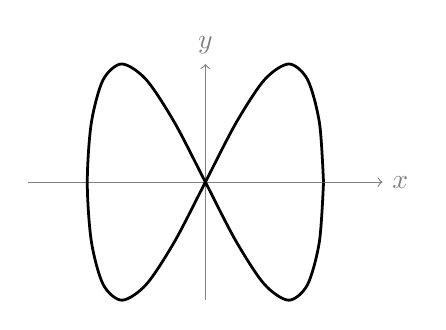
\begin{tikzpicture}[scale=1.5]
        \draw[->,gray] (-1.5,0) -- (1.5,0) node[right] {$x$};
        \draw[->,gray] (0,-1) -- (0,1) node[above] {$y$};
        \draw[line width=1pt] plot[smooth, domain=0:6.28] ({cos(\x r)},{sin(2*\x r)});
    \end{tikzpicture}
    \caption{浸入子流形的图像可能是一个自交的曲线}
\end{figure}

为了解决这个问题, 我们可以引入一个更强的概念, 即嵌入.

\begin{definition}[嵌入]
    设 $(f,M)$ 是 $N$ 的一个浸入子流形, 若 $f$ 是作为集合的映射是一个单射,
    且作为拓扑空间的映射 $f:M\to f(M)$ 是一个同胚, 则称 $(f,M)$ 是 $N$ 的一个{\bf 嵌入子流形} (embedded submanifold),
    或者简称为 $N$ 的一个{\bf 嵌入} (embedding).
\end{definition}

这种情况下, 嵌入的像就是一个完美的流形了. 这也是我们之所以这么定义的理由.

\begin{theorem}
    设 $f:M\to N$ 是一个单的浸入, 若 $M$ 紧致,
    则 $(f,M)$ 是 $N$ 的一个嵌入子流形. 
\end{theorem}
\begin{proof}
    由[\ref{thm:compact_to_hausdorff_homeomorphic}],
    则 $f:M\to f(M)$ 是一个同胚. 因此 $(f,M)$ 是 $N$ 的一个嵌入子流形.
\end{proof}

对应于此, 我们还有淹没的概念.

\begin{definition}[淹没]
    设 $M$ 是 $m$-光滑流形, $N$ 是 $n$-光滑流形,
    则一个光滑映射 $f:M\to N$ 称为{\bf 淹没} (submersion), 
    如果对于任意 $p\in M$, $f$ 都在 $p$ 处是非退化的. 
    
    此时称 $(f,M)$ 为 $N$ 的一个{\bf 淹没子流形} (submersed submanifold).
\end{definition}

\subsection{定向}

手性是线性空间中的一个重要概念. 他描述了一个线性空间的基底的方向.

\begin{definition}[定向]
    设 $V$ 是一个 $n$-维实线性空间, 则 $V$ 的{\bf 定向} (orientation) 定义为 $V$ 的所有基底的等价类,
    其中两组有序基底 $(v_1,\ldots,v_n)$ 和 $(w_1,\ldots,w_n)$ 等价, 如果存在一个线性变换 $A:V\to V$, 满足 $A(v_i)=w_i$ 对于任意 $i=1,\ldots,n$, 且 $\det A>0$.
\end{definition}

使用外代数的语言, 上述定义可以更简洁地表述为
\[(v_1,\ldots,v_n)\sim(w_1,\ldots,w_n)\iff\frac{w_1\wedge\cdots\wedge w_n}{v_1\wedge\cdots\wedge v_n}>0\]
显然这样的等价类只有两个, 因此我们可以说一个线性空间有两种手性, 分别称为左手和右手.
通过外代数的角度, 下面的定理可以很容易地证明.

\begin{theorem}
    设 $(v_1,\ldots,v_n)$ 是一组 $n$-实线性空间的基底,
    则任意调换两个基底向量 $v_i$ 和 $v_j$ 都会改变基底的手性. 
\end{theorem}

\begin{theorem}
    设 $(v_1,\ldots,v_n)$ 是一组 $n$-实线性空间的基底,
    则任意取反一个基底向量 $v_i$ 都会改变基底的手性.
\end{theorem}

我们希望将定向的概念推广到流形上. 由于流形的切空间是一个线性空间, 因此我们可以通过切空间的定向来定义流形的定向.
但是问题是如何对于每个点的切空间都选定统一的定向?
定向之间是否会互相冲突? 这都是我们感兴趣的内容.

\begin{definition}[定向的传播]
    设 $M$ 是 $m$-光滑流形, $\alpha:[0,1]\to M$ 是连续映射.
    并且在每一点 $\alpha(t)$ 都指定了 $T_{\alpha(t)}M$ 的定向
    $\mu_t$. 
    并且在每一点 $t_0$, $M$ 在 $\alpha_{t_0}$ 有容许坐标卡 $(U,\phi)$
    以及 $t_0$ 的邻域 $I=[t_0-\epsilon_1,t_0+\epsilon_2]$.
    (特别地, 当 $t_0=0$ 时, $\epsilon_1=0$; 当 $t_0=1$ 时, $\epsilon_2=0$).
    使得
    \[\alpha(I)\subset U\]
    并且
    \[\left(\frac{\del}{\del\phi^1}\Big|_{\alpha(t)}, \ldots, \frac{\del}{\del\phi^m}\Big|_{\alpha(t)}\right)\in\mu_t,
    \quad t\in I\]
    则称 $\mu$ 是沿着 $\alpha$ 的一个{\bf 定向的传播} (orientation propagation).

    显然, 设 $p,q\in M$ 是两点, $\alpha:[0,1]\to M$ 是连接 $p,q$ 的路径.
    在 $T_pM$ 中指定定向 $\mu_0=\lambda$, 则诱导了 $T_qM$ 中的一个定向 $\mu_1$,
    称 $\mu_1$ 是 $\lambda$ 沿着 $\alpha$ 传播到 $q$ 的结果.
\end{definition}

一个自然的问题是, 定向的传播是否会互相冲突? 不妨设 $M$ 道路连通,
那么对于任意两点 $p,q\in M$, 都存在连接 $p,q$ 的路径 $\alpha:[0,1]\to M$.
我们的问题是: 设两条不同的路径 $\alpha,\beta:[0,1]\to M$ 都连接 $p,q$, 那么他们
一定传播相同的定向吗?

一个经典的不能再经典的反例就是Möbius带.

\begin{figure}[htbp]
    \centering
    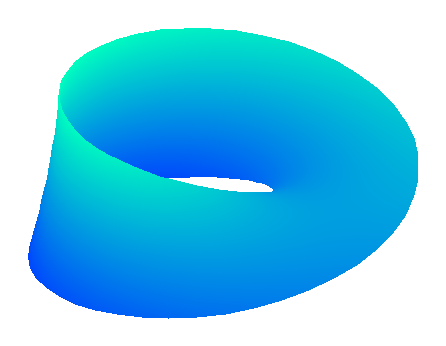
\begin{tikzpicture}
        \begin{axis}[
            axis equal,
            axis lines=none,
            shader=interp,
            colormap={cirno}{color(0cm)=(blue!75!cyan); color(1cm)=(cyan!75!green)},
        ]
            \addplot3[
                surf,
                domain=-1:1,
                domain y=-pi:pi,
                shader=interp,
                z buffer=sort,
                samples=18,
                samples y=48,
            ]({(2+x*cos(deg(y/2)))*cos(deg(y))},
            {(2+x*cos(deg(y/2)))*sin(deg(y))},
            {x*sin(deg(y/2))});
        \end{axis}
    \end{tikzpicture}
    \caption{Möbius带}
\end{figure}

上图是一个Möbius带, 设 $p$ 是图中间的点, 不妨考虑下图中的一条道路:

\begin{figure}[htbp]
    \centering
    \begin{tikzpicture}
        \begin{axis}[
            axis equal,
            axis lines=none,
            shader=interp,
            colormap={cirno}{color(0cm)=(blue!75!cyan); color(1cm)=(cyan!75!green)},
        ]
            \addplot3[
                mesh,
                domain=-1:1,
                domain y=-pi:pi,
                shader=interp,
                z buffer=sort,
                samples=18,
                samples y=48,
            ]({(2+x*cos(deg(y/2)))*cos(deg(y))},
            {(2+x*cos(deg(y/2)))*sin(deg(y))},
            {x*sin(deg(y/2))});
            \addplot3[
                only marks,
                mark=*,
                mark size=2pt,
                color=blue
            ] coordinates {
                (2, 0, 0)
            };
            \addplot3[
                samples y=100,
                domain y=-pi:pi,
                line width=1pt,
                black,
                samples=1,
                postaction={
                    decorate,
                    decoration={
                        markings,
                        mark=at position 0.25 with {\arrow[scale=1.5]{Stealth}},
                        mark=at position 0.75 with {\arrow[scale=1.5]{Stealth}},
                    }
                },
            ] ({2*cos(deg(y))}, {2*sin(deg(y))}, 0);
            \draw[line width=1.5pt,-{Latex},blue] (axis cs:2,0,0)--(axis cs:3,0,0);
            \draw[line width=1.5pt,-{Latex},dotted,blue] (axis cs:2,0,0)--(axis cs:1,0,0);
        \end{axis}
    \end{tikzpicture}
    \caption{Möbius带不可定向}
\end{figure}

该道路绕Möbius带的中线行驶一周, 最终得到的定向和原本相反. 因此这样的流形是存在的.
我们可以根据是否可以定向来对流形进行分类:

\begin{definition}[流形的定向]
    设 $M$ 是连通的流形, 若对于任意两点 $p,q\in M$, 以及连接 $p,q$ 的任意两条路径 $\alpha,\beta:[0,1]\to M$,
    都有 $\lambda$ 沿着 $\alpha$ 传播到 $q$ 的结果和 $\lambda$ 沿着 $\beta$ 传播到 $q$ 的结果相同, 
    则称 $M$ 是{\bf 可定向的} (orientable). 否则称 $M$ 是{\bf 不可定向的} (non-orientable).

    对于可定向的流形, 若指定了一个点的定向 $\lambda$, 
    那么这个定向可以唯一地传播到流形的每个点, 从而得到一个全局的定向 $\mu$.
    则称 $\mu$ 是 $M$ 的一个{\bf 定向} (orientation).
\end{definition}

\begin{theorem}[可定向的等价定义]
    设 $M$ 是一个连通的流形, 则 $M$ 可定向当且仅当对所有
    有交的坐标卡 $(U,\phi)$ 和 $(V,\psi)$ 以及点 $x\in U\cap V$,
    转移函数
    \[\psi\circ \phi^{-1}:\phi(U\cap V)\to\psi(U\cap V)\]
    的Jacobian行列式都是正的.
\end{theorem}
\begin{proof}
    该映射的Jacobian矩阵就是切映射的矩阵表示. 由[\ref{thm:jacobian_of_tangent_map}] 取 $f=\id$ 即知
    其为切空间上的切映射 $T_xM\to T_xM$ 的矩阵表示.
    
    该坐标变换将基底 $\set{\dfrac{\del}{\del \phi^1}\Big|_x,\ldots,\dfrac{\del}{\del \phi^m}\Big|_x}$ 映射到基底 $\set{\dfrac{\del}{\del \psi^1}\Big|_x,\ldots,\dfrac{\del}{\del \psi^m}\Big|_x}$
    从而其行列式为
    \[\frac{\dfrac{\del}{\del \psi^1}\Big|_x\wedge\ldots\wedge\dfrac{\del}{\del \psi^m}\Big|_x}
    {\dfrac{\del}{\del \phi^1}\Big|_x\wedge\ldots\wedge\dfrac{\del}{\del \phi^m}\Big|_x}\]
    因此该行列式为正当且仅当 $\set{\dfrac{\del}{\del \phi^1}\Big|_x,\ldots,\dfrac{\del}{\del \phi^m}\Big|_x}$ 和 $\set{\dfrac{\del}{\del \psi^1}\Big|_x,\ldots,\dfrac{\del}{\del \psi^m}\Big|_x}$ 具有相同的手性.
    从而对于任意两条连接 $p,q$ 的路径 $\alpha,\beta:[0,1]\to M$, $\lambda$ 沿着 $\alpha$ 传播到 $q$ 的结果和 $\lambda$ 沿着 $\beta$ 传播到 $q$ 的结果相同.
\end{proof}

\subsection{带边流形}

还记得我们一开始举的例子 $D^n$ 吗? 如果你注意力足够敏锐,
你会发现 $D^n$ 其实不符合我们之前定义的流形的定义. 因为 $D^n$ 的边界点没有邻域同胚于
$\R^n$. 但是 $D^n$ 又是一个非常重要的空间, 因此我们需要一个更广义的流形的定义来包含 $D^n$ 这样的空间. 这就是带边流形的定义.

我们先来讨论一个非常典型的空间, 即半空间 $H^n$. 其定义为
\[H^n=\set{(x^1,\ldots,x^n)\in\R^n\mid x^n\ge 0}\]
其上可以继承 $\R^n$ 的子空间拓扑. 显然其边界
\[\del H^n=\set{(x^1,\ldots,x^{n-1},0)\in\R^n\mid x^n=0}\]
是一个 $n-1$ 维的空间. $H^n$ 的内部
\[H^{n,\circ}=\set{(x^1,\ldots,x^n)\in\R^n\mid x^n>0}=H^n\setminus\del H^n\]
我们通过下面方法拓宽光滑函数的定义: 对于 $f:U\to\R$, 其中 $U\subset H^n$
是开子集, 若存在 $f':U'\to\R^n$ 是 $C^\dagger$ 函数,
其中 $U'$ 是 $\R^n$ 中的一个开子集, 满足 $U=U'\cap H^n$ 
以及 $f=f'|_U$, 则称 $f$ 是 $U$ 上的一个{\bf $C^\dagger$ 函数}.

此时, 若 $U$ 不包含边界点, 则 $C^\dagger$ 函数就是普通的光滑函数.

$H^n$ 的两个开子集 $U,V$ 之间的{\bf 光滑同胚}是指一个双射 $f:U\to V$,
使得 $f$ 和 $f^{-1}$ 都是 $C^\infty$ 函数. 即存在
$C^\dagger$ 函数 $f':U'\to V'$ 和 $g':V'\to U'$, 其中 $U',V'$ 是 $\R^n$ 中的开子集,
满足 $U=U'\cap H^n$, $V=V'\cap H^n$, $f=f'|_U$ 和 $f^{-1}=g'|_V$.

显然, $H^n$ 的微分同胚将内点映射到内点, 将边界点映射到边界点.

\begin{definition}[带边流形]
    
\end{definition}